\documentclass[border=4pt]{standalone}
\usepackage{fontspec}
\usepackage{amsmath}
\usepackage{unicode-math}
\setmainfont{Latin Modern Roman}
\setmathfont{Latin Modern Math}
\usepackage{pgfplots}
\usepackage{pgfplotstable}
\pgfplotsset{compat=1.18}
\usepackage{tkz-euclide}
\usetikzlibrary{arrows.meta,calc,angles,quotes,patterns,3d,backgrounds}
\definecolor{ink}{HTML}{123428}
\definecolor{asy}{HTML}{475569}
\definecolor{mint}{HTML}{86e0bd}
\tikzset{asym/.style={asy, line width=0.9pt, dash pattern=on 5pt off 3.5pt},
         guide/.style={gray!70, line width=0.6pt, densely dotted},
         dot/.style={circle, inner sep=0pt, minimum size=5pt, draw=white, line width=0.5pt},
         odot/.style={circle, inner sep=0pt, minimum size=5.5pt, fill=white, line width=1pt},
         lab/.style={font=\footnotesize, inner sep=1.5pt, text=ink}}
\begin{document}
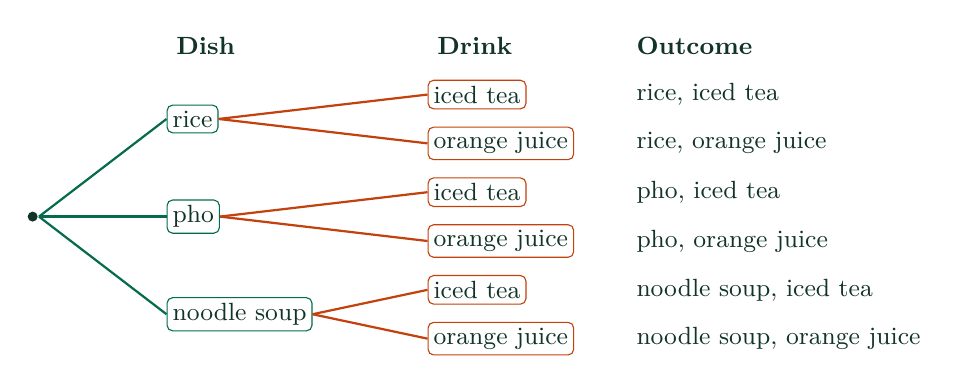
\begin{tikzpicture}
\fill[ink] (0,0) circle (1.8pt);
\node[draw={rgb,255:red,4;green,107;blue,77}, fill=white, rounded corners=2pt, inner sep=2pt, font=\small, text=ink, anchor=west] (a0) at (1.700,1.240) {rice};
\draw[color={rgb,255:red,4;green,107;blue,77}, line width=0.8pt] (0.08,0) -- (a0.west);
\node[draw={rgb,255:red,194;green,65;blue,12}, fill=white, rounded corners=2pt, inner sep=2pt, font=\small, text=ink, anchor=west] (b0) at (5.015,1.550) {iced tea};
\draw[color={rgb,255:red,194;green,65;blue,12}, line width=0.8pt] (a0.east) -- (b0.west);
\node[anchor=west, font=\small, text=ink] at (7.545,1.550) {rice, iced tea};
\node[draw={rgb,255:red,194;green,65;blue,12}, fill=white, rounded corners=2pt, inner sep=2pt, font=\small, text=ink, anchor=west] (b1) at (5.015,0.930) {orange juice};
\draw[color={rgb,255:red,194;green,65;blue,12}, line width=0.8pt] (a0.east) -- (b1.west);
\node[anchor=west, font=\small, text=ink] at (7.545,0.930) {rice, orange juice};
\node[draw={rgb,255:red,4;green,107;blue,77}, fill=white, rounded corners=2pt, inner sep=2pt, font=\small, text=ink, anchor=west] (a1) at (1.700,0.000) {pho};
\draw[color={rgb,255:red,4;green,107;blue,77}, line width=0.8pt] (0.08,0) -- (a1.west);
\node[draw={rgb,255:red,194;green,65;blue,12}, fill=white, rounded corners=2pt, inner sep=2pt, font=\small, text=ink, anchor=west] (b2) at (5.015,0.310) {iced tea};
\draw[color={rgb,255:red,194;green,65;blue,12}, line width=0.8pt] (a1.east) -- (b2.west);
\node[anchor=west, font=\small, text=ink] at (7.545,0.310) {pho, iced tea};
\node[draw={rgb,255:red,194;green,65;blue,12}, fill=white, rounded corners=2pt, inner sep=2pt, font=\small, text=ink, anchor=west] (b3) at (5.015,-0.310) {orange juice};
\draw[color={rgb,255:red,194;green,65;blue,12}, line width=0.8pt] (a1.east) -- (b3.west);
\node[anchor=west, font=\small, text=ink] at (7.545,-0.310) {pho, orange juice};
\node[draw={rgb,255:red,4;green,107;blue,77}, fill=white, rounded corners=2pt, inner sep=2pt, font=\small, text=ink, anchor=west] (a2) at (1.700,-1.240) {noodle soup};
\draw[color={rgb,255:red,4;green,107;blue,77}, line width=0.8pt] (0.08,0) -- (a2.west);
\node[draw={rgb,255:red,194;green,65;blue,12}, fill=white, rounded corners=2pt, inner sep=2pt, font=\small, text=ink, anchor=west] (b4) at (5.015,-0.930) {iced tea};
\draw[color={rgb,255:red,194;green,65;blue,12}, line width=0.8pt] (a2.east) -- (b4.west);
\node[anchor=west, font=\small, text=ink] at (7.545,-0.930) {noodle soup, iced tea};
\node[draw={rgb,255:red,194;green,65;blue,12}, fill=white, rounded corners=2pt, inner sep=2pt, font=\small, text=ink, anchor=west] (b5) at (5.015,-1.550) {orange juice};
\draw[color={rgb,255:red,194;green,65;blue,12}, line width=0.8pt] (a2.east) -- (b5.west);
\node[anchor=west, font=\small, text=ink] at (7.545,-1.550) {noodle soup, orange juice};
\node[font=\small\bfseries, text=ink, anchor=west] at (1.700,2.170) {Dish};
\node[font=\small\bfseries, text=ink, anchor=west] at (5.015,2.170) {Drink};
\node[font=\small\bfseries, text=ink, anchor=west] at (7.545,2.170) {Outcome};
\end{tikzpicture}
\end{document}
